\hypersetup{
    colorlinks=true,
    linkcolor=blue
}

\chapter{Introduction} \label{ch:introduction}
\begin{center}
  "We really designed the Model S to be a very sophisticated computer on wheels. We view this the same as updating your phone or your laptop. Tesla is a software company as much as it is a hardware company. A huge part of what Tesla is, is a Silicon Valley software company."
  - Elon Musk \cite{ElonMusk}
\end{center}
With these words, Elon Musk, the visionary entrepreneur behind many of the most innovative companies in today's business landscape and co-founder of one of, if not the, most progressive automotive companies of today, namely Tesla, highlighted how the automotive industry is changing dramatically over time, transforming today cars and vehicles from objects in which the fundamental part consists of mechanics components, to ones in which the main focus lies in the simplicity of hardware and the innovation of software.

This shift in paradigm, which is now a reality in the automotive industry, requires significant effort, especially from a security perspective. While a cyber vulnerability in a traditional device like a laptop or smartphone may result in data loss, vulnerabilities in a vehicle's computer system, where software is a fundamental element, can have tragic and even life-threatening consequences. For this reason, addressing security from the design stage is one of the primary objective of this paper.

In order to address and understand the Software Defined Vehicle, which is the most recent expression of software integration in the automobile, it is necessary to delve into the automotive industry and the dynamics that exist with respect to software production. For this reason, in this introduction an overview of the automotive context in which the project is located will be discussed and then the role of the project partner company, which is also a leader in software consulting and development and a partner of major automotive companies, will be detailed. Finally, in conclusion of this chapter, the thesis's key objectives and the practical project that will support this work during the description are shown.
\section{Context}
The automotive industry stands out as one of the fastest-growing sectors, playing a significant role as both an employer and an investor in research and development; at the same time, it represents one of the most crucial domains for the European Union's economy. As reported in the article \cite{automotiveInCentralEurope}, in 2015, 21 million motor vehicles of all types were produced in Europe, representing a 23\% share in the global production of more than 90 million units.

\begin{figure}[h]  % 'h' significa che la figura viene posizionata qui
  \centering
  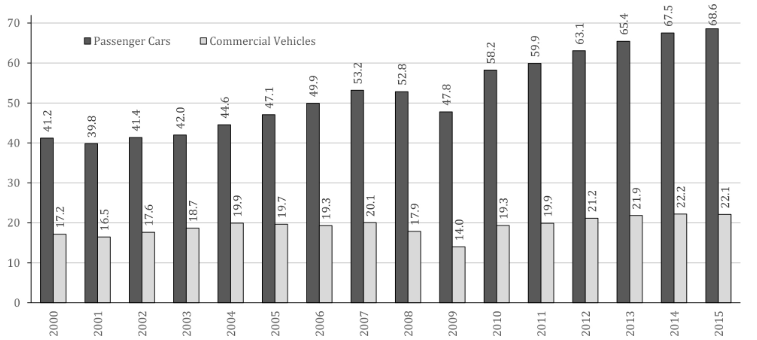
\includegraphics[width=0.9\textwidth]{images/automotive_world production.png}  % Sostituisci 'nome_immagine' con il nome del tuo file immagine e l'estensione
  \caption{World automobile production in million vehicles \cite{automotiveInCentralEurope}}
  \label{fig:WorldAutomobileProduction}
\end{figure}

In the evolving landscape of automotive technology, the imperative for automotive companies extends beyond the traditional realms of mechanical engineering to encompass a crucial reliance on both software and hardware components for vehicle construction. A glimpse into the intricate web of modern cars, as illustrated in Figure \ref{fig:VheicleProcessors}, reveals a mosaic of hundreds of distinct processors interfacing at various levels, earning contemporary vehicles the moniker of "Computers on wheels."

\begin{figure}[h]  % 'h' significa che la figura viene posizionata qui
  \centering
  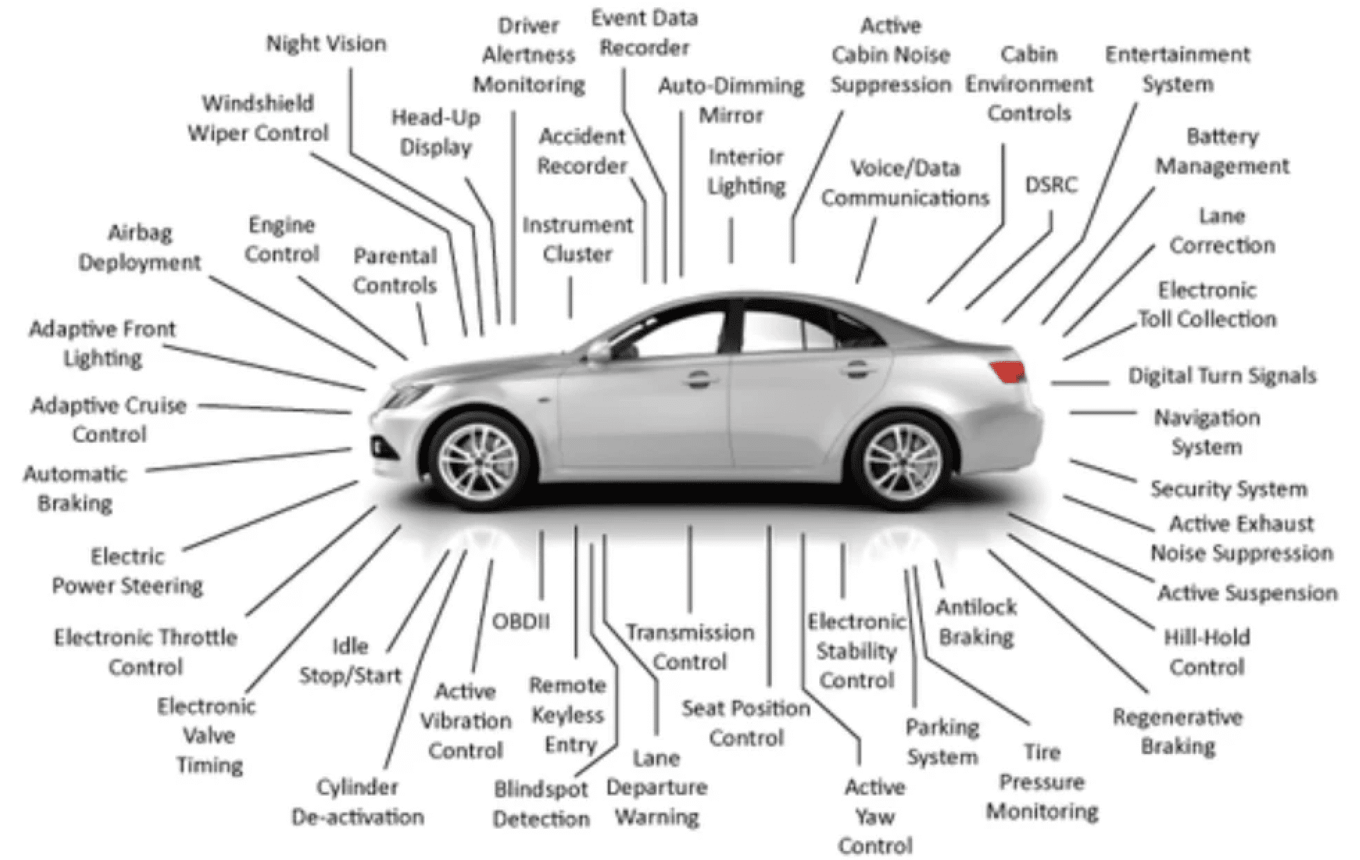
\includegraphics[width=0.9\textwidth]{images/vehicle_processors.png}  % Sostituisci 'nome_immagine' con il nome del tuo file immagine e l'estensione
  \caption{An incomplete overview of computers in a modern car \cite{ieeeSoftwareDefinedVehicle}}
  \label{fig:VheicleProcessors}
\end{figure}

However, the proliferation of processors within vehicles, orchestrating communication to manage diverse components, presents a formidable challenge; each component often integrates a processor with unique logics, diverging from the logics embedded in processors of other components. Complicating matters further, these components are frequently supplied by companies with proprietary management logics, not readily accessible to the automotive companies themselves.

In addressing this intricate scenario, the transformative concept of a Software Defined Vehicle (SDV) comes to the forefront. Defined as "any vehicle that manages its operations, adds functionality, and enables new features primarily or entirely through software"  \cite{blackberrySDV}, the notion of SDV offers a comprehensive solution to the challenges posed by the intricate interplay of software and hardware in modern vehicles.

Effectively navigating the development of SDV technology necessitates a collaborative approach across diverse companies, particularly in the realms of hardware and cloud computing. This collaborative synergy is exemplified in the realization of our project, made possible through the partnership with Storm Reply.


\section{Company}

Leveraging extensive experience in the cloud industry and fostering deep-rooted relationships within the automotive sector, Storm Reply stands out as the ideal choice to lead the project discussed in this thesis. A key player in the Reply group, Storm Reply specializes in designing and implementing innovative Cloud-based solutions and services \cite{StormReplySite}. 

With a diverse clientele spanning various sectors, notably the automotive industry, the company's expertise played a pivotal role in comprehensively understanding the project's context and internal dynamics. This profound knowledge served as the cornerstone for developing a tangible exemplification of the infrastructure.

\begin{figure}[h]  % 'h' significa che la figura viene posizionata qui
  \centering
  
\includegraphics[width=0.3\textwidth]{images/Storm_Reply_logo.png}  % Sostituisci 'nome_immagine' con il nome del tuo file immagine e l'estensione
  \caption{Logo of the partenr company of the project}
  \label{fig:StormReplyLogo}
\end{figure}

A point of pride for Storm Reply is its recognition as an Amazon Web Services (AWS) Premier Consulting Partner since 2014, ranking among the top Amazon Partners globally. This distinctive characteristic underscores the decision to develop the infrastructure using Amazon Web Services.

According to the official AWS description page \cite{AWSGlobalInfrastructure} the AWS Cloud spans 102 Availability Zones within 32 geographic Regions around the world and servs 245 countries and territories. With millions of active customers and tens of thousands of partners globally, AWS has the largest and most dynamic ecosystem. AWS is evaluated as a Leader in the 2022 Gartner Magic Quadrant for Cloud Infrastructure and Platform Services, placed highest in Ability to Execute axis of measurement among the top 8 vendors named in the report.

\begin{figure}[h]  % 'h' significa che la figura viene posizionata qui
  \centering
  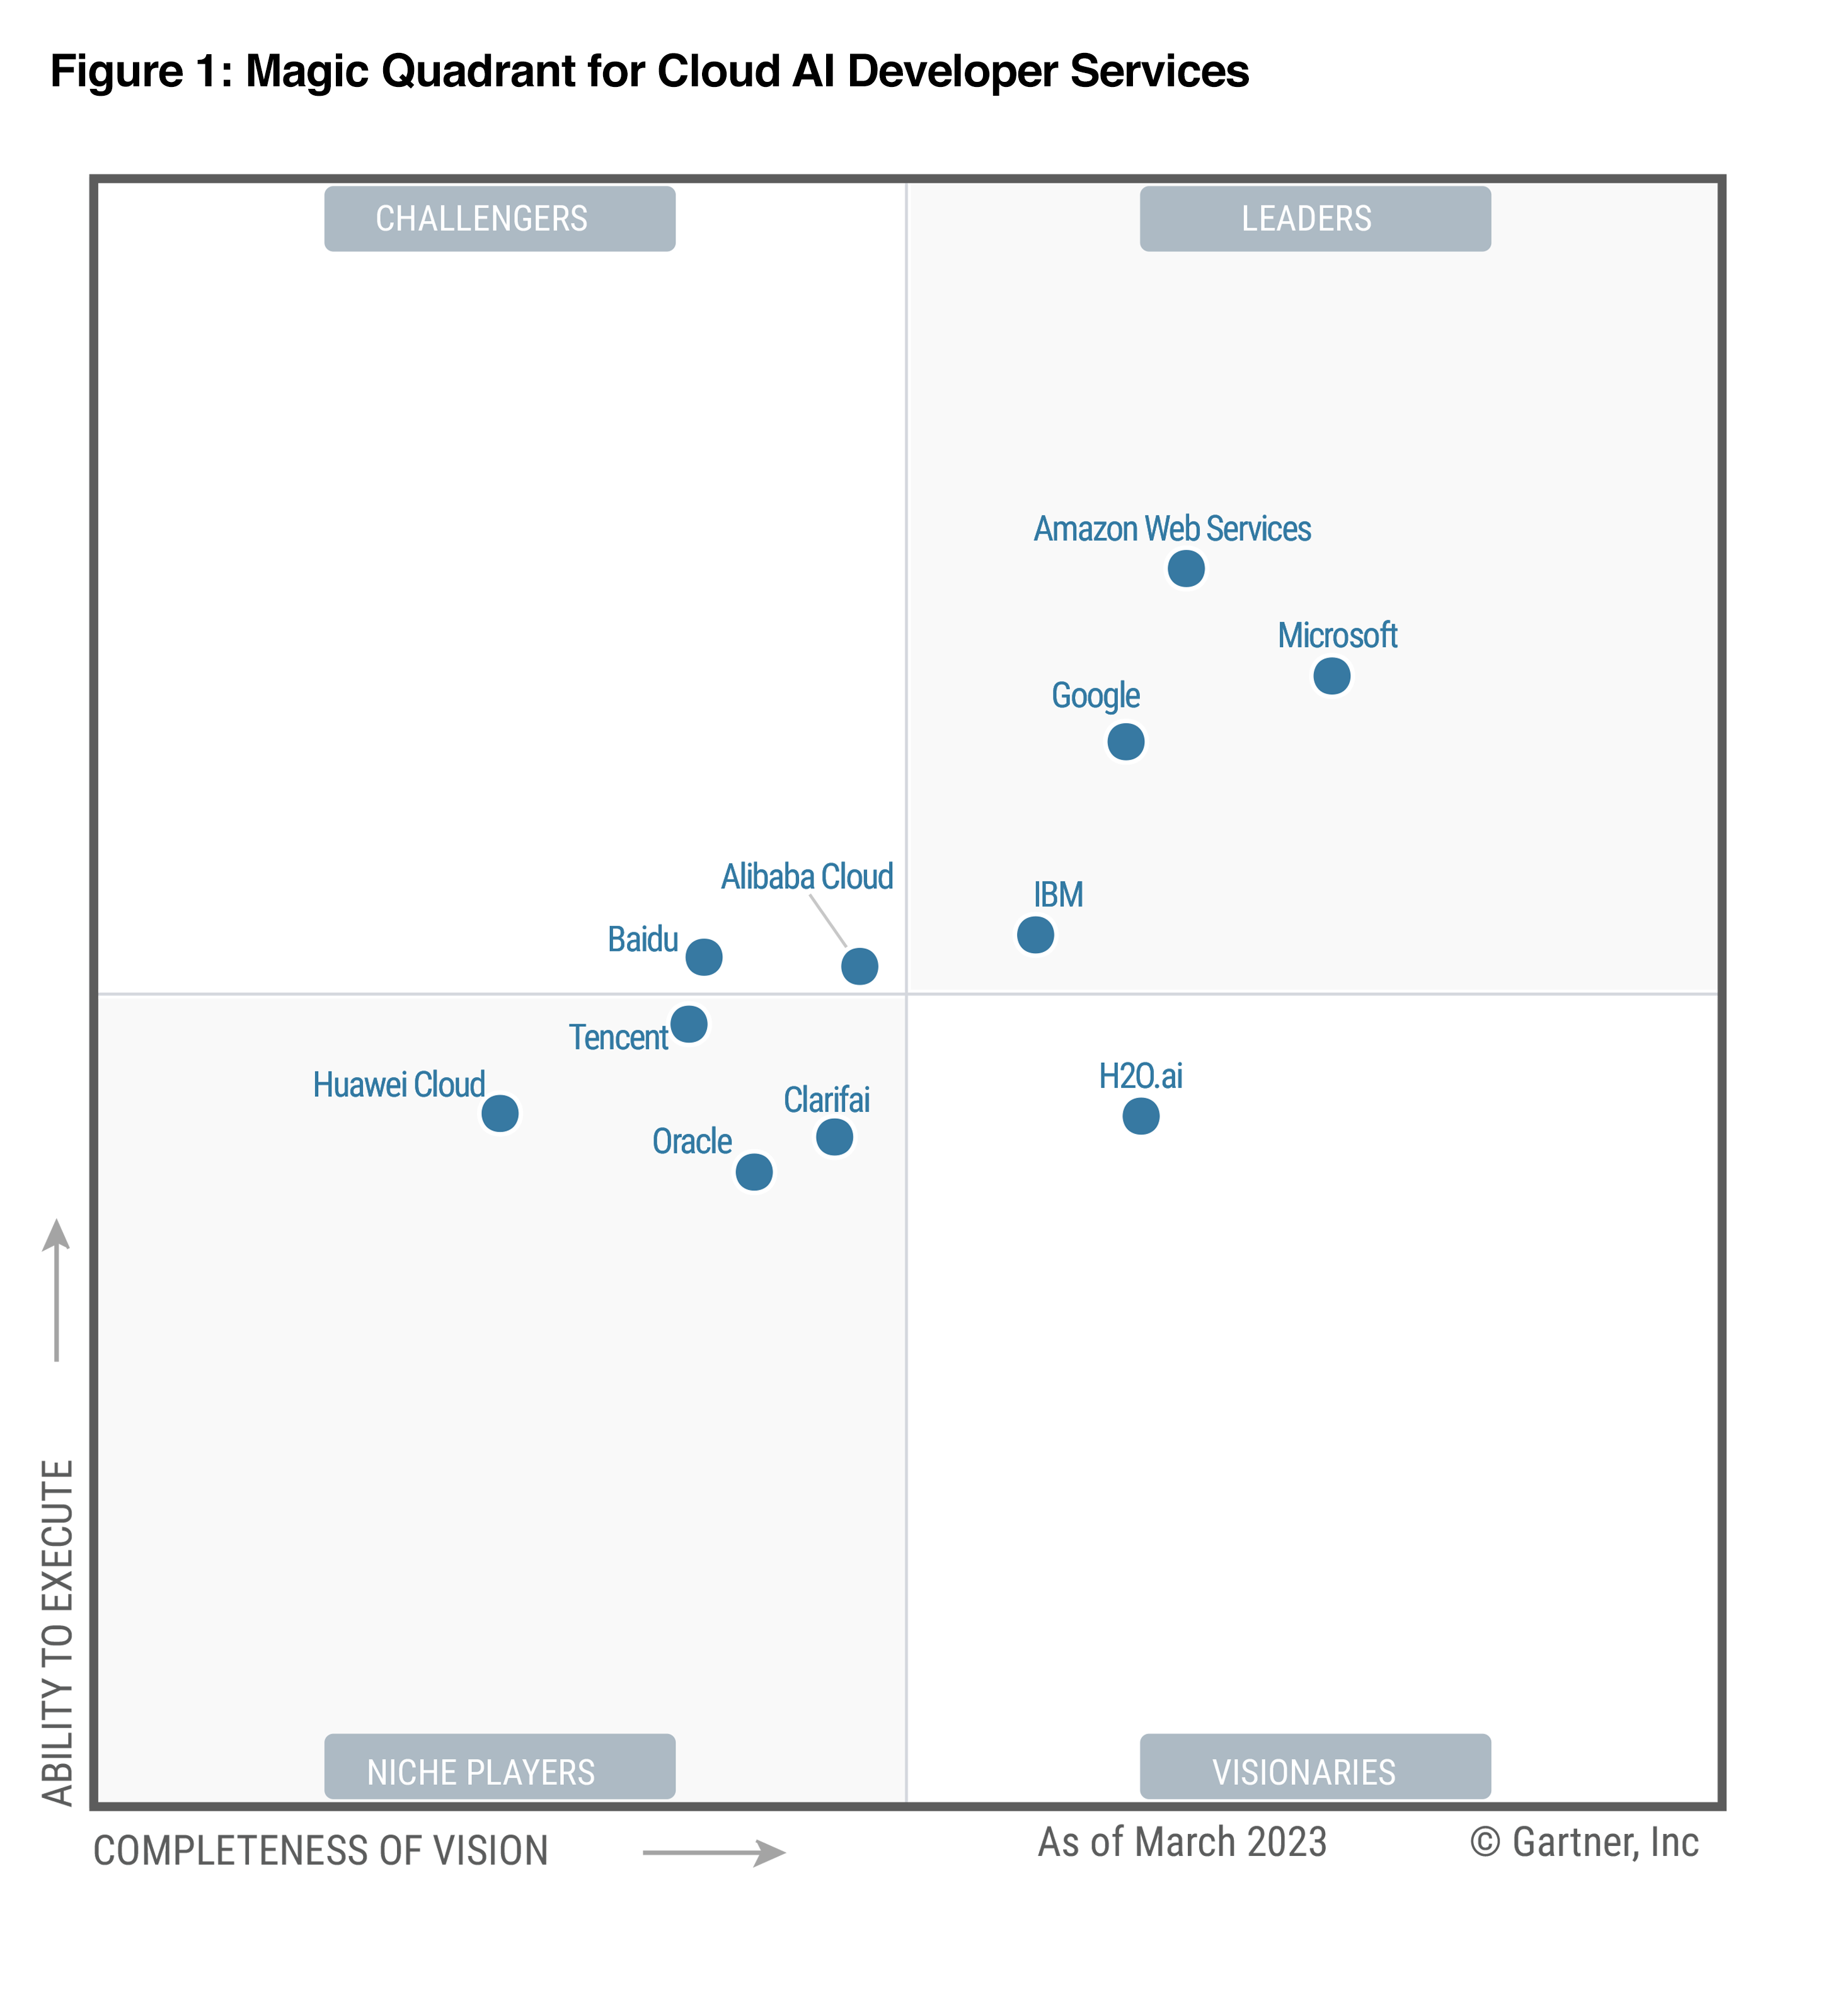
\includegraphics[width=0.3\textwidth]{images/AWSMagicQuadrantForCloud.png}  % Sostituisci 'nome_immagine' con il nome del tuo file immagine e l'estensione
  \caption{Here are a series of market research reports published by IT consulting firm Gartner that rely on proprietary qualitative data analysis methods to demonstrate market trends, such as direction, maturity and participants. \cite{GartnerMagicQuadrant}}
  \label{fig:AWSMagicQuadrantForCloud}
\end{figure}

The infrastructure exhibits several key attributes contributing to its robustness and efficiency: 
\begin{itemize} 
  \item \textbf{Security:} The infrastructure undergoes 24/7 monitoring to ensure the confidentiality, integrity, and availability of data. All data flowing across the AWS global network is automatically encrypted at the physical layer before leaving secured facilities.
  \item \textbf{Availability:} To ensure high availability and isolate potential issues, applications can be partitioned across multiple AZs (Availability Zones) within the same region, creating fully isolated infrastructure partitions.
  \item \textbf{Performance:} AWS Regions offer low latency, low packet loss, and high overall network quality. This is achieved through a fully redundant 100 GbE fiber network backbone, often providing terabits of capacity between Regions.
  \item \textbf{Scalability:} The AWS Global Infrastructure allows companies to take advantage of the virtually infinite scalability of the cloud. This enables customers to provision resources based on actual needs, with the ability to instantly scale up or down according to business requirements.
  \item \textbf{Flexibility:} The AWS Global Infrastructure provides flexibility in choosing where and how workloads are run, whether globally, with single-digit millisecond latencies, or on-premises.
  \item \textbf{Global Footprint:} AWS boasts the largest global infrastructure footprint, continually expanding at a significant rate.
\end{itemize}

\section{Thesis Goal}
In the automotive context, the use of Software Defined Vehicle (SDV) plays a crucial role in terms of costs, innovation, and safety. The goal of the thesis intertwine with the opportunities provided by Software Defined Vehicle technology, addressing the primary challenge of managing the current difficulties associated with the presence of various specialized hardware platforms on the same vehicle.

The central objective of this thesis is to propose a Software Defined Vehicle solution capable of eliminating various phases of the software production pipeline. This would result in significant time and cost savings, enabling the investment of these resources in other sectors. Since, by definition, a Software Defined Vehicle is characterized by the ability to undergo software updates dynamically and flexibly, this solution offers significant security advantages in various aspects:
\begin{enumerate}
  \item Human Safety Critical Security: From the moment that a vehicle can be classified as safety critical (as it is reported in the standard ISO 26262-1:2018 of the ISO society where is said that "safety is one of the key issues in the development of road vehicles" \cite{ISO26262}), the elimination of software vulnerabilities related to the vehicle's systems is crucial for the overall safety of the vehicle itself.  
  \item Intrinsic Software Security: This approach allows for the prevention and resolution of vulnerabilities unknown at the time of software design, contributing to ensuring a high standard of security.
\end{enumerate}

Consequently, the use of Software Defined Vehicle aims to completely separate software and hardware, allowing the production of high-level software on entirely generalized hardware systems. This results in significant savings in terms of time and money for hardware production, along with providing an advantage in terms of security due to the simplification of software.

For example, as demonstrated by NIST in the research on the Analysis Of The Impact Of Software Complexity \cite{NISTCodeComplexity}, the increase in software complexity in different cases results in less analyzable programs. In some instances, the same vulnerability analysis tool may detect vulnerabilities, while in others, analyzing the same code, it may not. 

From a practical standpoint, the project's goal is to provide, through the use of AWS services, a cloud infrastructure capable of managing the Software Defined Vehicle both in terms of software production and data analysis.